\documentclass[letterpaper]{book}
\usepackage{makeidx}
\usepackage{fancyheadings}
\usepackage{epsfig}
\usepackage{graphics,color}
\usepackage{float}
\usepackage{doxygen}
\makeindex
\setcounter{tocdepth}{1}
\setlength{\footrulewidth}{0.4pt}
\begin{document}
\begin{titlepage}
%\setlength{\epsfxsize}{\textwidth}
%\epsffile{../petra.eps}
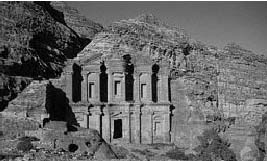
\includegraphics{../epetra.eps}
\begin{center}
{\Huge Trilinos/Petra: Linear Algebra Services Package\\[1ex]\large Version 2.0}\\
\vspace*{1cm}
{\large Written by Michael A. Heroux, Robert J. Hoekstra and Alan
Williams}\\
\vspace*{0.5cm}
{\small November 2001}\\
\copyright Sandia National Laboratories 2001
\end{center}
\end{titlepage}
\clearemptydoublepage
\pagenumbering{roman}
\tableofcontents
\clearemptydoublepage
\pagenumbering{arabic}
\chapter{Overview of the Trilinos/Petra Package}
\input{index}

